\documentclass[journal,12pt,twocolumn]{IEEEtran}

\usepackage{setspace}
\usepackage{gensymb}

\singlespacing


\usepackage[cmex10]{amsmath}

\usepackage{amsthm}

\usepackage{mathrsfs}
\usepackage{txfonts}
\usepackage{stfloats}
\usepackage{bm}
\usepackage{cite}
\usepackage{cases}
\usepackage{subfig}

\usepackage{longtable}
\usepackage{multirow}

\usepackage{enumitem}
\usepackage{mathtools}
\usepackage{steinmetz}
\usepackage{tikz}
\usepackage{circuitikz}
\usepackage{verbatim}
\usepackage{tfrupee}
\usepackage[breaklinks=true]{hyperref}
\usepackage{graphicx}
\usepackage{tkz-euclide}
\usepackage{float}

\usetikzlibrary{calc,math}
\usepackage{listings}
    \usepackage{color}                                            %%
    \usepackage{array}                                            %%
    \usepackage{longtable}                                        %%
    \usepackage{calc}                                             %%
    \usepackage{multirow}                                         %%
    \usepackage{hhline}                                           %%
    \usepackage{ifthen}                                           %%
    \usepackage{lscape}     
\usepackage{multicol}
\usepackage{chngcntr}

\DeclareMathOperator*{\Res}{Res}

\renewcommand\thesection{\arabic{section}}
\renewcommand\thesubsection{\thesection.\arabic{subsection}}
\renewcommand\thesubsubsection{\thesubsection.\arabic{subsubsection}}

\renewcommand\thesectiondis{\arabic{section}}
\renewcommand\thesubsectiondis{\thesectiondis.\arabic{subsection}}
\renewcommand\thesubsubsectiondis{\thesubsectiondis.\arabic{subsubsection}}


\hyphenation{op-tical net-works semi-conduc-tor}
\def\inputGnumericTable{}                                 %%

\lstset{
%language=C,
frame=single, 
breaklines=true,
columns=fullflexible
}
\begin{document}


\newtheorem{theorem}{Theorem}[section]
\newtheorem{problem}{Problem}
\newtheorem{proposition}{Proposition}[section]
\newtheorem{lemma}{Lemma}[section]
\newtheorem{corollary}[theorem]{Corollary}
\newtheorem{example}{Example}[section]
\newtheorem{definition}[problem]{Definition}

\newcommand{\BEQA}{\begin{eqnarray}}
\newcommand{\EEQA}{\end{eqnarray}}
\newcommand{\define}{\stackrel{\triangle}{=}}
\bibliographystyle{IEEEtran}
\providecommand{\mbf}{\mathbf}
\providecommand{\pr}[1]{\ensuremath{\Pr\left(#1\right)}}
\providecommand{\qfunc}[1]{\ensuremath{Q\left(#1\right)}}
\providecommand{\sbrak}[1]{\ensuremath{{}\left[#1\right]}}
\providecommand{\lsbrak}[1]{\ensuremath{{}\left[#1\right.}}
\providecommand{\rsbrak}[1]{\ensuremath{{}\left.#1\right]}}
\providecommand{\brak}[1]{\ensuremath{\left(#1\right)}}
\providecommand{\lbrak}[1]{\ensuremath{\left(#1\right.}}
\providecommand{\rbrak}[1]{\ensuremath{\left.#1\right)}}
\providecommand{\cbrak}[1]{\ensuremath{\left\{#1\right\}}}
\providecommand{\lcbrak}[1]{\ensuremath{\left\{#1\right.}}
\providecommand{\rcbrak}[1]{\ensuremath{\left.#1\right\}}}
\theoremstyle{remark}
\newtheorem{rem}{Remark}
\newcommand{\sgn}{\mathop{\mathrm{sgn}}}
\providecommand{\abs}[1]{\left\vert#1\right\vert}
\providecommand{\res}[1]{\Res\displaylimits_{#1}} 
\providecommand{\norm}[1]{\left\lVert#1\right\rVert}
%\providecommand{\norm}[1]{\lVert#1\rVert}
\providecommand{\mtx}[1]{\mathbf{#1}}
\providecommand{\mean}[1]{E\left[ #1 \right]}
\providecommand{\fourier}{\overset{\mathcal{F}}{ \rightleftharpoons}}
%\providecommand{\hilbert}{\overset{\mathcal{H}}{ \rightleftharpoons}}
\providecommand{\system}{\overset{\mathcal{H}}{ \longleftrightarrow}}
	%\newcommand{\solution}[2]{\textbf{Solution:}{#1}}
\newcommand{\solution}{\noindent \textbf{Solution: }}
\newcommand{\cosec}{\,\text{cosec}\,}
\providecommand{\dec}[2]{\ensuremath{\overset{#1}{\underset{#2}{\gtrless}}}}
\newcommand{\myvec}[1]{\ensuremath{\begin{pmatrix}#1\end{pmatrix}}}
\newcommand{\mydet}[1]{\ensuremath{\begin{vmatrix}#1\end{vmatrix}}}
\numberwithin{equation}{subsection}
\makeatletter
\@addtoreset{figure}{problem}
\makeatother
\let\StandardTheFigure\thefigure
\let\vec\mathbf
\renewcommand{\thefigure}{\theproblem}
\def\putbox#1#2#3{\makebox[0in][l]{\makebox[#1][l]{}\raisebox{\baselineskip}[0in][0in]{\raisebox{#2}[0in][0in]{#3}}}}
     \def\rightbox#1{\makebox[0in][r]{#1}}
     \def\centbox#1{\makebox[0in]{#1}}
     \def\topbox#1{\raisebox{-\baselineskip}[0in][0in]{#1}}
     \def\midbox#1{\raisebox{-0.5\baselineskip}[0in][0in]{#1}}
\vspace{3cm}
\title{Assignment3}
\author{SOWMYA BANDI}
\maketitle
\newpage
\bigskip
\renewcommand{\thefigure}{\theenumi}
\renewcommand{\thetable}{\theenumi}
Download all python codes from 
\begin{lstlisting}
https://github.com/Sowmyabandi99/Assignment3/tree/main/Assignment3/Assignment3
\end{lstlisting}
%
and download all latex-tikz codes from 
%
\begin{lstlisting}
https://github.com/Sowmyabandi99/Assignment3/blob/main/Assignment3/main.tex
\end{lstlisting}
%
\section{Question No. 2.16}
Find the direction vectors  and y-intercepts of the following lines.
\begin{enumerate}
%\begin{multicols}{2}
\item
\begin{align}
\begin{split}
\myvec{1 & 7}\vec{x}&=0  \label{eq1}
\end{split}
\end{align}
\item
\begin{align}
\begin{split}
\myvec{6 & 3}\vec{x}&=5  \label{eq2}
\end{split}
\end{align}
\item
\begin{align}
\begin{split}
\myvec{0 & 1}\vec{x}&=0  \label{eq3}
\end{split}
\end{align}
%\end{multicols}
\end{enumerate}
%
\section{Solution}
\begin{lemma}
\label{lemma}
Direction vector and y-intercept of the line $\vec{n}^T\vec{x}=c$ are:
\\
Direction vector
\begin{align}
\vec{m}= \myvec{b \\ -a}
\end{align}
and
\\
y-intercept = $\frac{c}{\vec{n}^T\vec{e_2}}$ $\quad(\because \vec{e_2}=\myvec{0\\1})$
\end{lemma}
\begin{enumerate}
%\begin{multicols}{2}
\item From the given line $\myvec{1 & 7}\vec{x}=0$,we have
\begin{align}
a=1,b=7,c=0
\end{align}
Normal vector
\begin{align}
\begin{split}
\vec{n} = \myvec{1 \\ 7}
\end{split}
\end{align}
Direction vector
\begin{align}
\vec{m} = \myvec{7 \\ -1}
\end{align}
y-intercept = \myvec{0 \\ 0}
\\
PLOT OF THE GIVEN LINE:
\numberwithin{figure}{section}
\begin{figure}[ht!]
Plot of \eqref{eq1} -
\centering
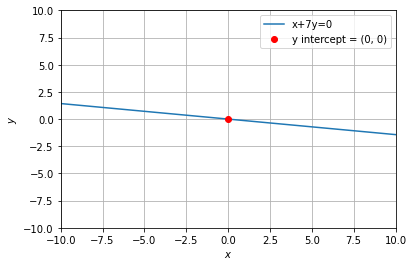
\includegraphics[width=\columnwidth,height=5 cm]{Fig1.png}
\caption{Figure1}
\end{figure}
\item From the given line $\myvec{6 & 3}\vec{x}=5$,we have
\begin{align}
a=6,b=3,c=5
\end{align}
Normal vector
\begin{align}
\begin{split}
\vec{n} = \myvec{6 \\ 3}
\end{split}
\end{align}
Direction vector
\begin{align}
\vec{m} = \myvec{3 \\ -6}
\end{align}
y-intercept = $\frac{5}{3}\vec{e_2}$   
\\
PLOT OF THE GIVEN LINE:
\numberwithin{figure}{section}
\begin{figure}[ht!]
Plot of \eqref{eq2}
\centering
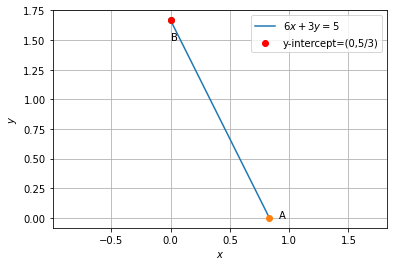
\includegraphics[width=\columnwidth,height=4 cm]{Fig2.png}
\caption{Figure2}
\end{figure}
\item From the given line $\myvec{0 & 1}\vec{x}=0$,we have
\begin{align}
a=0,b=1,c=0
\end{align}
Normal vector
\begin{align}
\begin{split}
\vec{n} = \myvec{0 \\ 1}
\end{split}
\end{align}
Direction vector
\begin{align}
\vec{m} = \myvec{1 \\ 0}
\end{align}
y-intercept = \myvec{0 \\ 0}
\\
PLOT OF GIVEN LINE:
\numberwithin{figure}{section}
\begin{figure}[ht!]
Plot of \eqref{eq3} -
\centering
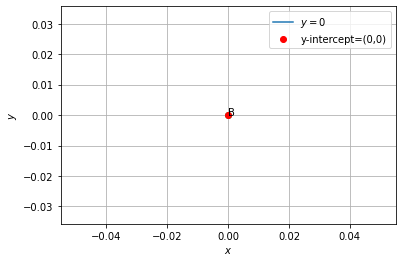
\includegraphics[width=\columnwidth]{Fig3.png}
\caption{Figure3}
\end{figure}
%\end{multicols}
\end{enumerate}
\end{document}